\documentclass[10pt,letterpaper]{article}
\usepackage{apacite}
\usepackage{cogsci}
\usepackage{color}
\usepackage{graphicx}
\usepackage{amssymb,amsmath,amsthm,amsfonts}
\usepackage{hyperref}
\title{Helping people choose subgoals with sparse pseudo rewards}

\author{
Frederick Callaway \\
Dept. of Psychology, UC Berkeley\\
\texttt{fredcallaway@berkeley.edu} \\
}

\newcommand{\fix}{\marginpar{FIX}}
\newcommand{\new}{\marginpar{NEW}}

\begin{document}
\newcommand{\NParticipant}{88}
\newcommand{\BetaRate}{-0.049}
\newcommand{\WorsenRate}{2.21}
\newcommand{\AovRateNull}{$\chi^2(3)=nan,\ nan$}
\newcommand{\AovRateFull}{$\chi^2(4)=12.62,\ p\,<\,0.001$}
\newcommand{\BetaThree}{0.169}
\newcommand{\ImprovementThree}{8.51}
\newcommand{\AovThreeNull}{$\chi^2(3)=nan,\ nan$}
\newcommand{\AovThreeFull}{$\chi^2(4)=5.61,\ p\,<\,0.05$}


\maketitle


\section{Introduction}\label{introduction}

Many important decisions require sacrificing immediate reward in the pursuit of greater payoffs in the future. However, planning far into the future involves considering an exponentially increasing number of possible paths. Even in constrained games such as Go or Chess, no computer can consider every possible sequence of moves. The computational complexity of planning far into the future may partially explain the fact that people tend to underappreciate future rewards relative to immediate rewards \cite{Myerson1995}.

Inspired by the use of \emph{shaping rewards} in reinforcement learning \cite{ng99}, \citeA{LiederGriffiths2016} showed that this problem can be ameliorated by providing people with \emph{pseudo-rewards} that align short term reward with long term value. However, in the real world it is infeasible to give people pseudo-rewards in response to every one of their decisions. Can we attain a similar benefit from providing pseudo-rewards with less frequency? Here, we provide empirical evidence that \emph{sparse pseudo-rewards} can also improve performance, but that this benefit declines as the spacing between pseudo-rewards increases.



\section{Methods} % (fold)
\label{methods}
We recruited \NParticipant~participants on Amazon's Mechanical Turk. Participants navigated a spider through the \emph{Web of Cash} (Figure~\ref{fig:paradigm}), attempting to collect the maximum amount of money. The web was structured such that participants could only move rightwards, and only one row up or down on each step. This induces a long-term planning problem in which one may need to make a short-term suboptimal decision to reach a highly valuable state. On some trials, pseudo-rewards, displayed as stars, were presented every 1, 2, or 3 steps. Only the pseudo-rewards at the nearest such column were visible; when one of those pseudo-rewards was attained, the next round appeared. Participants were explicitly informed that the number of stars on a state was the maximum total profit one could gain starting in that state.


\begin{figure}[t!]
\begin{minipage}{.47\textwidth}
    %\centering
    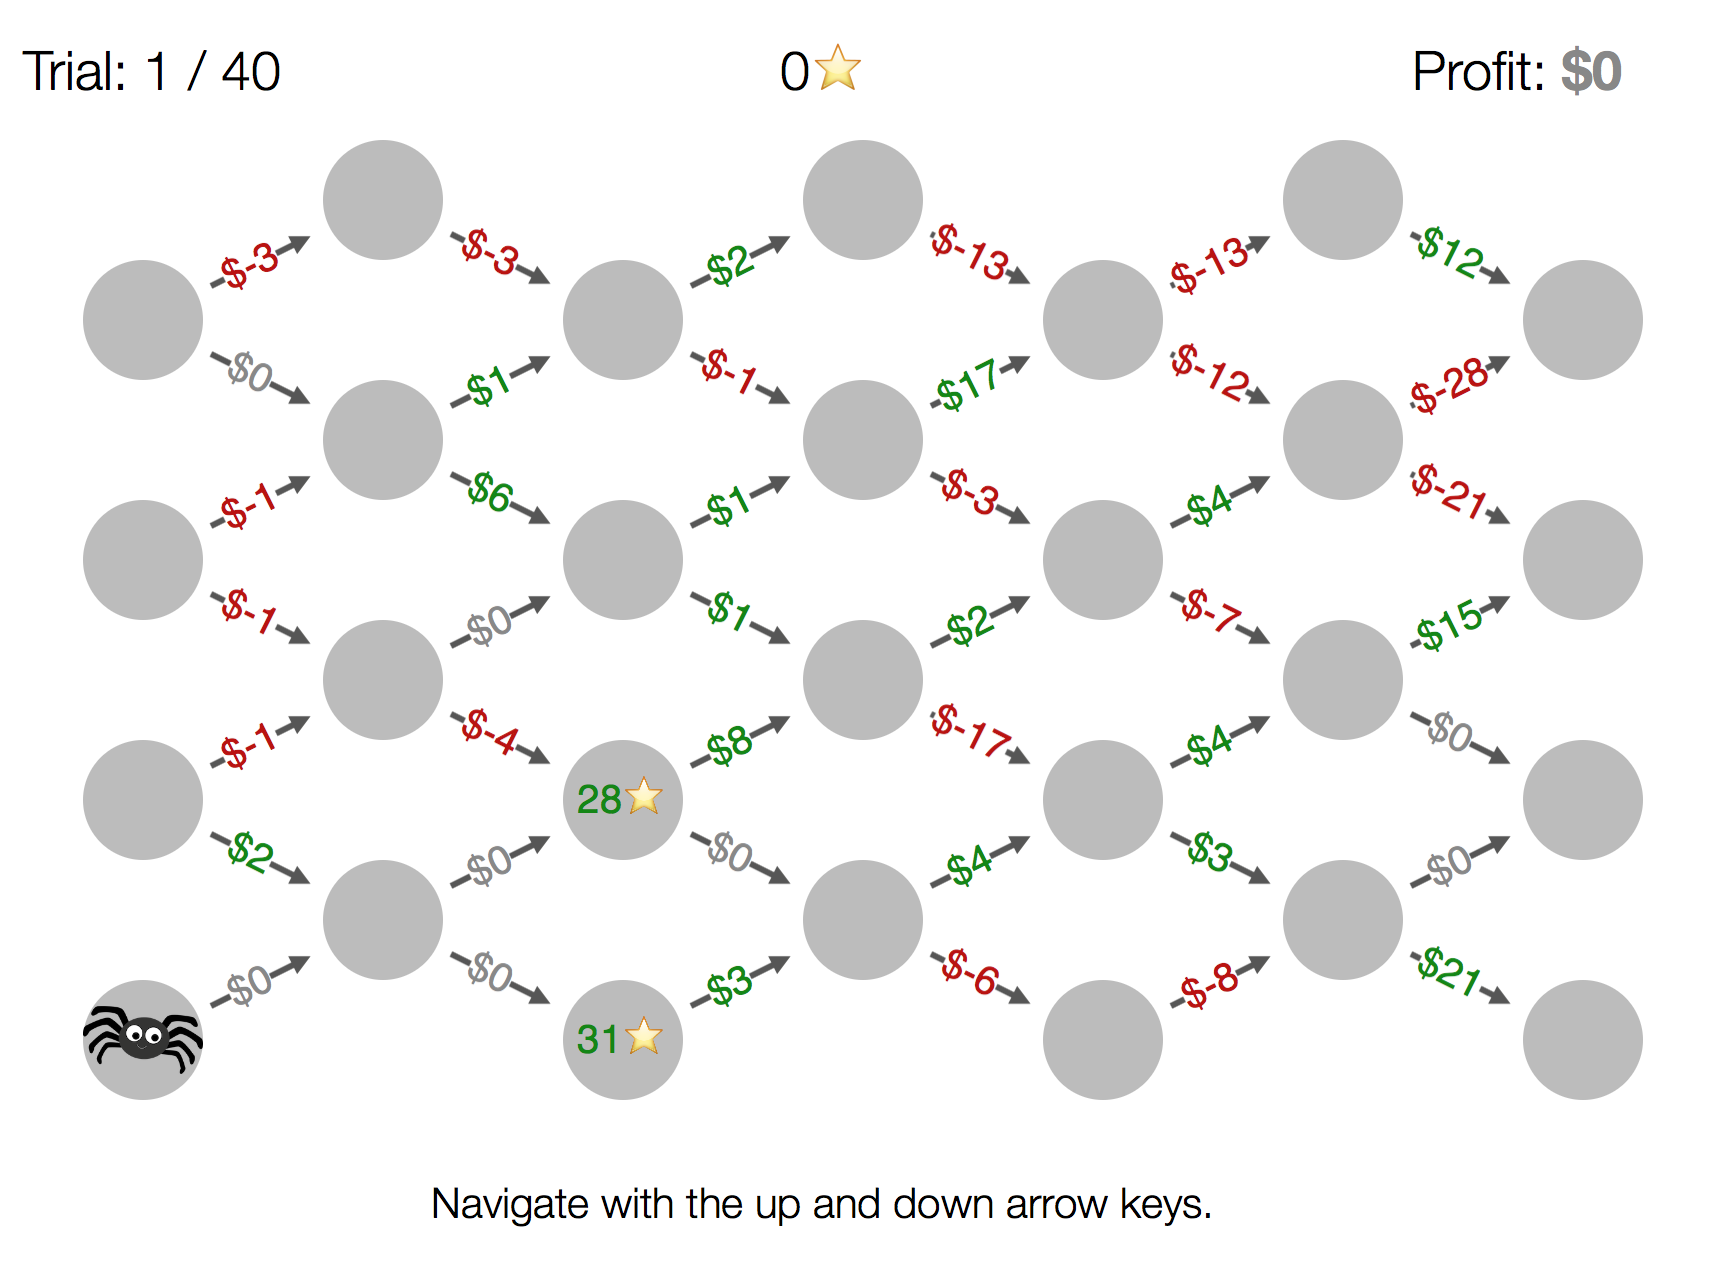
\includegraphics[width=\linewidth]{figs/paradigm.png}
    \caption{Screenshot of the experiment: Participants control the spider with the arrow keys to maximize profit. The number of stars conveys the value of a state.}
    \label{fig:paradigm}
\end{minipage}%
\begin{minipage}{.1\textwidth}
$\;\;$
\end{minipage}
\begin{minipage}{.455\textwidth}
  %\centering
  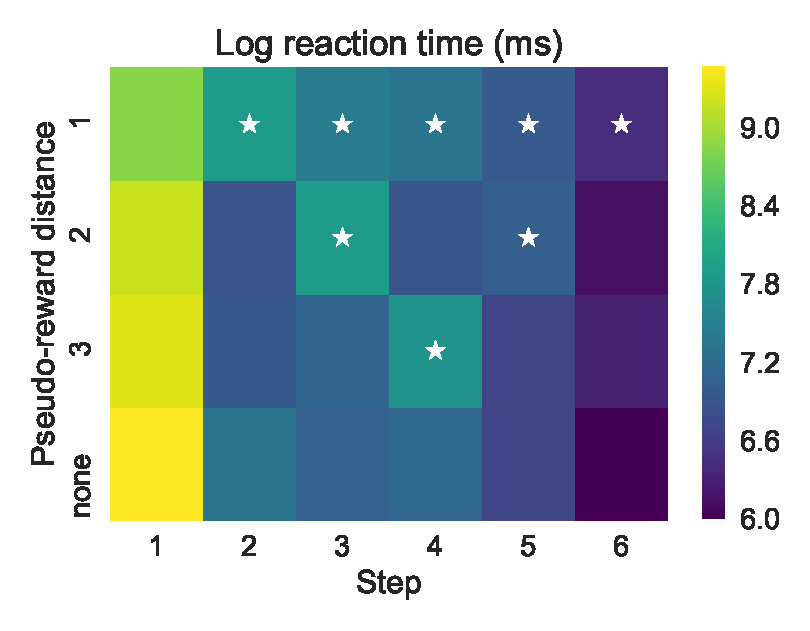
\includegraphics[width=\linewidth]{figs/plan_time.eps}
  \caption{Planning time is higher on states with pseudo-rewards, indicated by stars.}
  \label{fig:plan-time}
\end{minipage}
\end{figure}


\begin{figure*}[t!]
    \centering
    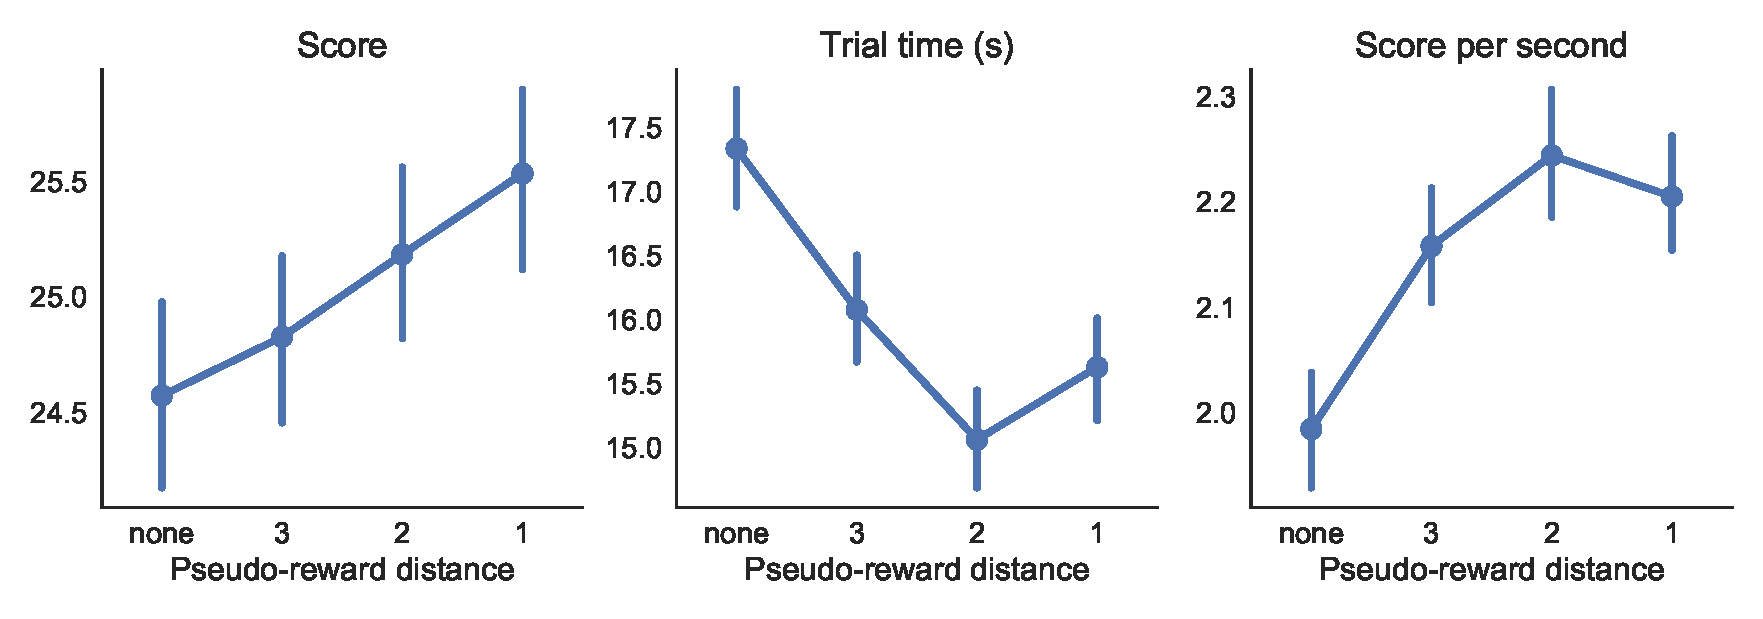
\includegraphics[width=0.85\textwidth]{figs/basic.eps}
    \caption{Average score, trial time, and score rate (score per second) for different frequencies of pseudo-rewards. Error bars show 68\% confidence intervals by bootstrapping.}
    \label{fig:basic}
\end{figure*}

\section{Results}\label{results}

Data and analysis code can be viewed at \url{https://github.com/fredcallaway/psych205/}

\subsection{Score rate}
We predicted that pseudo-rewards would either increase the quality of actions, reduce the time spent planning, or both. To capture both of these possibilities in one metric, we defined \emph{score rate} to be the average score per second. Results are plotted in Figure~\ref{fig:basic}.

\subsubsection{Model description}
For each measure (score, time, score rate), we constructed a mixed effects linear regression model with one fixed effect for distance between pseudo-rewards (or 6, the number of steps, when pseudo-rewards were absent) and one random effect for participant. This corresponds to the following equation

\begin{equation}
    \hat{y} = \beta_0 + \beta_1 x_{p,t} + \beta_p + \epsilon_{p,t}
\end{equation}

where $\beta_0$ is the intercept, $\beta_1$ is the fixed effect, $x_{p,t}$ is the pseudo-reward distance on trial $t$ for participant $p$, $\beta_p$ is the random intercept for each participant, and $\epsilon_{p,t}$ is the error term which is drawn from a Normal distribution with a separate variance for each participant. That is:

\begin{equation}
    \epsilon_{p,t} \sim \text{N}(0, \sigma^2_p)
\end{equation}

This model assumes that mean score rate is a linear function of the distance between pseudo-rewards, after adjusting for differences in participant's mean score rates. For each participant, adjusted individual score rates will be Normally distributed around this mean, although individual participants may differ in how much they vary from the mean on each trial.

The difference between the greatest pseudo-reward distance (every three steps) and the absence of pseudo-reward is especially interesting. Thus, we constructed a model similar to the one above, but restricting the data to trials on which either 3-step or no pseudo-rewards were shown. In this case, our predictor variable $x_{p,t}$ is a factor indicating whether or not pseudo-rewards were present.


\subsubsection{Model results} % (fold)

We found a small effect of pseudo-reward distance ($\beta = \BetaRate$), corresponding to a \WorsenRate\% decrease in score rate for each additional step between pseudo-rewards. This is in line with our prediction that increasing distance between pseudo-rewards would decrease score rate.

To test for significance, we used an Anova to compare the full model to a null model that only accounted for the global intercept and participant-level differences. Assuming the null hypothesis that there is no effect of pseudo-rewards, the difference in deviance (sum squared errors in this case) should be distributed according to $\chi^2(1)$. The Anova revealed that the effect of pseudo-rewards was significant (\AovRateFull).

Looking at only the difference between the 3-step and absent pseudo-reward trials, we see a stronger effect ($\beta = \BetaThree$; \AovThreeFull) corresponding to a \ImprovementThree\% improvement due to the presence of 3-step pseudo-rewards. 


\subsection{Reaction times}\label{planning-time}

In our second analysis, we sought evidence that the pseudo-rewards induced goal-targeted planning. We defined an intuitive behavioral signature of planning based on reaction times: If a participant chooses to plan ahead at a given state, her reaction time will be higher than average; however, once a plan has been formed, she can quickly execute the full sequence. Thus, if the pseudo-rewards induced subgoal-targeted planning, we would expect to see longer reaction times on states with pseudo-rewards because participants would need to re-plan after reaching the pseudo-reward induced subgoal. Log reaction times broken down by step and pseudo-reward frequency are shown in Figure~\ref{fig:plan-time}. We excluded the first action (the first column in Figure~\ref{fig:plan-time}) from our analysis because one would expect unusually high reaction time at the first state regardless of the presence of pseudo-rewards.


\subsubsection{Permutation test}

Although log reaction times are well approximated by a Normal distribution, we used a one-way permutation test with 10,000 samples because, hey—why not? This revealed a highly significant effect of pseudo-rewards on planning time ($p < .001$).


\section{Conclusion}\label{discussion}

We found that pseudo-reward induced subgoals enabled people to solve sequential decision problems more efficiently, suggesting that pseudo-rewards could be used in real-world settings to help people make better decisions. However, this benefit diminished as the distance between pseudo-rewards increased, suggesting that a decision-support application that employs pseudo-rewards should aim to provide pseudo-rewards as frequently as is feasible.

The effect of pseudo-rewards, while significant, was somewhat weak. In future work we will explore more complex domains in which pseudo-rewards have a greater potential to improve performance


%\bibliographystyle{Science}
\bibliographystyle{apacite}
\renewcommand{\bibliographytypesize}{\small}
% \setlength{\bibleftmargin}{.05in}
% \setlength{\bibindent}{-\bibleftmargin}
% \bibliography{references,Master}
\bibliography{references}

\end{document}